\documentclass[11pt]{article}

\usepackage[T1]{fontenc}
\usepackage[utf8]{inputenc}
\usepackage[english]{babel}
\usepackage[margin=1in]{geometry}
\usepackage{lmodern}
\usepackage{microtype}
\usepackage{mathtools}
\usepackage{amsmath,amssymb,amsthm}
\usepackage{array}
\usepackage{booktabs}
\usepackage{tabularx}
\usepackage{float}
\usepackage{graphicx}
\usepackage{pdflscape}
\usepackage{caption}
\usepackage{enumitem}
\usepackage{fancyhdr}
\usepackage[numbers]{natbib}
\usepackage{doi}
\usepackage{xurl}
\usepackage{hyperref}
\usepackage{cleveref}
\usepackage{orcidlink}
\usepackage{titling}

%--- paper-local packages ---
% longtable is required by the generated tables under tables/out/.
\usepackage{longtable}

% Shared manuscript macros for the paper.
% Stable, cross-section macros — keep wording mechanically enforced via these.
% Add macros incrementally as new vocabulary stabilizes during drafting; never redefine locally.

%--- claim pinning -----------------------------------------------------------
% \claimref{ROW_ID}{SHA256}: pins a claims-ledger row + one of its cited artifact hashes at the
% citation site. The hash argument is NOT rendered (it would be noise in running prose); it is a
% machine-checkable pin that tests/test_paper_gates.py verifies against paper/claims_ledger.json
% and the current artifact bytes. Never hand-edit the hash without re-running
% experiments/check_claims_ledger.py.
\newcommand{\claimref}[2]{[#1]}

%--- citation discipline -----------------------------------------------------
% \sbtcite{KEY}: thin wrapper so SBT-corpus citations are visually distinguishable in the source
% from literature citations, even though both compile through the same .bib file.
\newcommand{\sbtcite}[1]{\cite{#1}}

%--- nonclaims ---------------------------------------------------------------
\newcommand{\nonclaim}[1]{\par\noindent\textit{Nonclaim:} #1\par}

\input{includes/release_metadata}

\newtheorem{theorem}{Theorem}[section]
\newtheorem{lemma}[theorem]{Lemma}
\newtheorem{proposition}[theorem]{Proposition}
\newtheorem{corollary}[theorem]{Corollary}
\theoremstyle{definition}
\newtheorem{definition}[theorem]{Definition}
\newtheorem{remark}[theorem]{Remark}
\floatstyle{ruled}
\newfloat{algorithm}{tbp}{loa}
\floatname{algorithm}{Algorithm}

\urlstyle{same}
\captionsetup{
  font=small,
  labelfont=bf,
  labelsep=period
}
\captionsetup[table]{skip=6pt,position=top}
\captionsetup[figure]{skip=6pt}
\captionsetup[algorithm]{skip=6pt,position=top}
\crefname{algorithm}{algorithm}{algorithms}
\Crefname{algorithm}{Algorithm}{Algorithms}
\crefname{theorem}{theorem}{theorems}
\Crefname{theorem}{Theorem}{Theorems}
\crefname{lemma}{lemma}{lemmas}
\Crefname{lemma}{Lemma}{Lemmas}
\crefname{proposition}{proposition}{propositions}
\Crefname{proposition}{Proposition}{Propositions}
\crefname{corollary}{corollary}{corollaries}
\Crefname{corollary}{Corollary}{Corollaries}
\crefname{definition}{definition}{definitions}
\Crefname{definition}{Definition}{Definitions}
\crefname{remark}{remark}{remarks}
\Crefname{remark}{Remark}{Remarks}
\setlist[enumerate]{leftmargin=*, itemsep=2pt, topsep=4pt}
\setlength{\droptitle}{-3.2em}
\pretitle{\begin{center}\LARGE\bfseries}
\posttitle{\par\end{center}\vspace{0.5em}}
\preauthor{\begin{center}\normalsize}
\postauthor{\par\end{center}\vspace{-0.4em}}
\predate{\begin{center}\small}
\postdate{\par\end{center}\vspace{0.6em}}
\setlength{\emergencystretch}{2em}
\clubpenalty=10000
\widowpenalty=10000
\displaywidowpenalty=10000
\interfootnotelinepenalty=10000
\allowdisplaybreaks[2]
\fancypagestyle{firstpage}{\fancyhf{}
  \fancyfoot[C]{\scriptsize Automorph Inc., Wilmington, DE, USA \quad \texttt{ioannis@automorph.io} \quad \textcopyright\ \manuscriptyear \quad CC-BY 4.0}
  \renewcommand{\headrulewidth}{0pt}
  \renewcommand{\footrulewidth}{0pt}
}

\title{Glass Is an Unclosed Layer:\\
  Kovacs Memory as Predictive-Quotient Residue}
\author{Ioannis Tsiokos\,\orcidlink{0009-0009-7659-5964}}
\date{\manuscriptdate\quad\manuscriptversion\\[0.3em]
  \ifpaperhasdoi DOI: \href{https://doi.org/\paperdoi}{\paperdoi}\fi}
\hypersetup{
  pdftitle={Glass Is an Unclosed Layer: Kovacs Memory as Predictive-Quotient Residue},
  pdfauthor={Ioannis Tsiokos},
  hidelinks
}

\begin{document}

\maketitle
\thispagestyle{firstpage}

\begin{abstract}
Sixty years of searching have produced no universally accepted static order parameter for glass,
and the Kovacs crossover experiment of 1963 illustrates the difficulty: at the crossing moment the glass equals
its equilibrium in the monitored quantity and then departs from it, so that quantity alone does
not fix what happens next. We turn that observation into theorems on a small, exactly computable
class of kinetically constrained models (East, Fredrickson--Andersen, and a Bouchaud-type trap
family), where kernels, stationary measures, witnesses, and zero controls are ratios of integers
and the remaining certificate evidence is deterministic float64, labeled as such in each
artifact. The question we make precise is whether a declared readout forms a \emph{closed}
description: whether its present value determines its own future statistics. On the declared
scope we show: the energy readout of an aging East chain is far from closed, its closure deficit
exceeding the constrained-equilibrium baseline by a certified margin of $3/2$ (achieved
$\approx 1.64$), and that baseline is itself provably nonzero, because closure is a property of
the kinetic constraint rather than of equilibrium (GT1); the Kovacs protocol yields an exact pair
of preparation histories with identical present mean energy and different futures (GT2); all
$512$ yes/no functions of the declared energy readout agree on such a pair while a finer readout
of the same microstate separates it, so no static order parameter built from the energy readout
separates, on that class, what the pair's futures separate (GT3); five constructed look-alike
regimes are correctly rejected by the same classifier that accepts the Kovacs candidate (GT4);
one added scalar coordinate, a fictive-temperature-like index among others, resolves the pair,
which demonstrates the repair mechanism without proving that one scalar is insufficient in
general (GT5); the description of histories by future-equivalence strictly extends the declared
energy-based description, certified for the audited shell (GT6);
and aging constants frozen on East and transferred to FA under a pre-registered no-fitting protocol
scored 8 passes and 14 one-sided failures, with the trap family unobservable for a reason we
prove: the declared trap weight family's stationary distribution is exactly temperature-invariant
(GT7). A vendored Lean core machine-checks the abstract witness and refinement theorems;
attempting to encode the numeric witness produced a machine-checked impossibility theorem that
locates that core's expressiveness boundary. Every claim is hash-pinned to its artifacts, and the
full ledger of what is \emph{not} claimed is printed unabridged.
\end{abstract}

\medskip
\noindent\textbf{Keywords.} glass transition; Kovacs effect; aging and memory; kinetically
constrained models; East model; fictive temperature; closure deficit; lumpability; predictive
quotient; Six Birds Theory; emergence calculus; exact finite certificates; pre-registered
prediction; Lean.

% Manuscript inputs.
\section{Introduction}
\label{sec:intro}
%% Packet W-11 (first half; written last, from the frozen results sections, per
%% design/paper_plan.md and paper/narrative.md). Readability pass 2026-09-22: rewritten for a
%% glass-physics reader; claims unchanged.

\subsection{The problem}

Anderson called the nature of glass and the glass transition probably the deepest and most
interesting unsolved problem in solid-state theory \cite{anderson-1995}. One face of that problem is sixty years old and
unusually concrete: no universally accepted static order parameter for glass has emerged. A glass and a liquid
can agree in density, energy, and every routinely monitored one-time observable, yet behave
differently \cite{debenedetti-stillinger-2001}; conventional low-order static correlations show no
clear signature of the transition, and the candidate structural measures that do grow remain
contested \cite{berthier-biroli-2011,cavagna-2009,tarjus-2011,royall-williams-2015}. A second face has sat in the laboratory record since 1963: Kovacs's
crossover experiment \cite{kovacs-1963}. Equilibrate a polymer glass hot, quench it, age it, then
jump the temperature up and watch its volume relax. At some moment the volume \emph{equals} its
new equilibrium value, and does not stay there: it overshoots through a non-monotone hump before
returning. At the crossing moment the sample is indistinguishable from equilibrium in the
monitored observable and distinguishable from it in its future, a point made explicit at the
level of configurations in simulation \cite{mossa-sciortino-2004}. The standard partial fix, the
Tool--Narayanaswamy--Moynihan fictive temperature \cite{tool-1946,narayanaswamy-1971,moynihan-1976},
adds one memory variable; richer protocols expose the limits of any single such variable and
have motivated multiparameter models \cite{ritland-1956,kahr-1979,hodge-1994,mckenna-simon-2017}. Memory effects
of this kind, in which a material's response depends on its history in a way no monitored
one-time observable records, are now studied across many classes of matter \cite{keim-2019}.

\subsection{The question, made precise}

Both faces are the same question. Take a declared readout of the system (here, the energy of a
spin chain; in the laboratory, the volume) and ask: \emph{is that readout a closed description of
the dynamics?} A readout is closed over a horizon $\tau$ if its present value determines the
statistics of its value $\tau$ steps later, so that a law can be written in the readout's
vocabulary without loss, the informational closure of \cite{bertschinger-2006,pfante-2014}. In Markov-chain language the readout is closed at horizon $\tau$ exactly
when the $\tau$-step readout transition probabilities agree across every populated microstate with
the same readout, which for a fully supported distribution is lumpability of the readout
\cite{burke-rosenblatt-1958,kemeny-snell-1960}. In this paper a static order-parameter candidate is taken in one operational sense only: a
function of the declared readout that separates two preparations whose futures differ. Any
function of the readout that fails to separate them (a constant does so trivially) cannot carry
the information the futures carry, and that is the sense in which GT3 below forecloses the
search: not that no coarsening of the energy is closed, but that none of them tells the exhibited
pair apart. That is narrower than the field's usage. The Kovacs hump is a direct demonstration
that the monitored volume is not closed.

Once the question is put this way, three further questions become computable on a finite model.
How far from closed is the readout, in nats? Can one exhibit a concrete certificate of the
failure, that is, two preparation histories that agree on the readout now and differ in their
futures? And is there \emph{any} function of the readout that recovers the missing predictive
distinction, or must it be carried by a genuinely new coordinate, and at what cost?

\subsection{What this paper does}

We answer those questions on a class of models small enough that the certificates are exact
ratios of integers wherever the artifact declares them so, and deterministic float64 elsewhere:
kinetically constrained models
\cite{ritort-sollich-2003,garrahan-sollich-toninelli-2011}, with the East model
\cite{jackle-eisinger-1991} as the substrate on which everything is built and calibrated, and
the Fredrickson--Andersen model \cite{fredrickson-andersen-1984} and a Bouchaud-type trap family
\cite{bouchaud-1992,monthus-bouchaud-1996} as out-of-sample transfer targets. At the system sizes
used ($N \le 10$ spins for certificates), transition kernels, stationary measures, witness pairs,
and zero controls are ratios of integers; the closure-deficit grid of GT1 is deterministic
float64 and is labeled as such in its artifact, with its margin far from the rounding scale. The
price is that every result is a statement about a declared finite class of models, sizes,
observables, and protocols, and we state that scope in every claim.

The bookkeeping that keeps those scopes honest is borrowed from a certificate-based closure
calculus, Six Birds Theory \sbtcite{sbt-primer,sbt-foundations-i,sbt-foundations-ii,%
sbt-foundations-iii,sbt-foundations-iv,sbt-paper-a,sbt-paper-b,sbt-paper-c}. The reader does not
need that corpus to follow this paper: \S\ref{sec:methods} defines every object we use in
ordinary probabilistic terms, and the framework's own labels appear only where a claim is filed in
its vocabulary, always with a plain gloss. Readers who want the formal anchors will find each
claim's corpus reference in the claims ledger shipped with the paper.

The results, each at its declared scope (\S\ref{sec:gt1}--\S\ref{sec:gt7}), read as follows.

\begin{itemize}
  \item \textbf{GT1, the energy readout is not closed.} For an aging East chain, the closure
    deficit of the energy readout (the conditional mutual information between the microstate now
    and the energy later, given the energy now) exceeds the same quantity at constrained
    equilibrium by a certified factor of at least $3/2$. A correction to our own design
    expectations came with it: the equilibrium value is provably \emph{not} zero, because
    closure depends on where the mobile excitations sit, not on whether the chain is stationary.
  \item \textbf{GT2, the Kovacs witness.} The Kovacs protocol on East yields an exact pair of
    preparation histories with the same present mean energy and different future mean energies
    under the declared continuation.
  \item \textbf{GT3, the order-parameter search is foreclosed on the declared class.} Every one of
    the $512$ yes/no functions definable from the declared energy readout agrees on a witness
    pair that a finer readout of the same microstate (the occupation of the site next to the
    wall) separates. On that class, no static order parameter built from the energy readout can
    do the job; whatever does the job must carry information the energy readout does not.
  \item \textbf{GT4, the kill-test panel.} The classifier that accepts the Kovacs memory
    candidate correctly rejects five constructed look-alike regimes, schematic fixtures for a
    protocol artifact, dissipation, an explicitly latent variable, an equilibrium control, and an
    incomplete continuation catalog.
  \item \textbf{GT5, the cost of repair.} One added scalar coordinate resolves the witness pair,
    and a fictive-temperature-like index (the index of the grid point whose equilibrium mean energy is closest to each
    microstate's energy, averaged over the history) is one of three that do. The
    certificate shows the repair mechanism on this pair; it does not prove that one scalar is
    insufficient in general.
  \item \textbf{GT6, the memory layer is strictly richer.} The description of histories by
    future-equivalence strictly extends the declared energy-based description, certified for the
    audited shell (the frozen set of eligibility conditions, \S\ref{sec:methods}) by an explicit
    gate table and ablation panel.
  \item \textbf{GT7, aging constants transfer only partly.} Six aging readouts were frozen on
    East, predictions for FA and the trap family were pre-registered, and the targets were then
    run and scored mechanically: 8 of 22 scored predictions passed, 14 failed on the same side,
    and the trap family produced no Kovacs hump at all, for a reason we prove.
\end{itemize}

Two further results come from the formalization effort (\S\ref{sec:lean}). A vendored core of
the framework's theorems is machine-checked in the Lean proof assistant, and the attempt to encode
the numeric Kovacs witness in that core produced a machine-checked impossibility theorem instead,
which locates exactly which certificates can live in that core and why.

\subsection{How to read the claims}

Four contributions, in the order we would defend them. First, the \textbf{discipline}: every
claim quantifies over a declared finite class, is pinned by content hash to the artifact that
supports it, is accompanied by controls, and is filed together with what it does \emph{not}
assert; honest negatives are results, and the discipline forced several of our own claims to
shrink. Second, the \textbf{result complex} itself: seven claims, four bridges, and six honest
negatives, each hash-pinned to its artifacts. The bracketed labels throughout, such as [GT1], are
machine-checked citations into the claims ledger, not decoration. Third, the
\textbf{freeze-and-transfer protocol with its actual scoreboard}: the failures are results, with
a clean one-sided pattern and a proven structural explanation for the empty column. Fourth, the
\textbf{Lean-checked core and the scope-boundary finding}.

What this paper is not: it proves nothing about all glasses, the continuum, or the ideal-glass
transition; it makes no irreversibility claims; and its field-facing sentence, ``no static order
parameter,'' is licensed only over the declared class it is proved on. The full list of nonclaims
is printed, unabridged, in \S\ref{sec:discussion}.

\section{Definitions and Methods}
\label{sec:methods}
%% Packet W-01. No claims-ledger rows attach here directly; background + certificate discipline.
%% Readability pass 2026-09-22: objects defined in ordinary probabilistic terms first; framework
%% labels kept as anchors.

\subsection{The objects, in plain terms}

Everything in this paper is built from a finite-state Markov chain and a choice of what to
observe. Five objects carry all seven results; we define each in ordinary terms, with the Kovacs
experiment as the running example, and give its source in the Six Birds Theory (SBT) corpus, which
we cite rather than re-derive \sbtcite{sbt-primer,sbt-foundations-i,sbt-foundations-ii,%
sbt-foundations-iii,sbt-foundations-iv,sbt-paper-a,sbt-paper-b,sbt-paper-c}.

\begin{description}[leftmargin=1.5em, itemsep=4pt]
  \item[Lens.] The observable panel: a map $f$ from the microstate space $Z$ to a finite set of
    readout values. Our main lens is the energy readout $L_{\mathrm{energy}}$, the number of up
    spins; the ``thermodynamic lens'' $\Pi_{\mathrm{std}}$ is this readout together with its
    declared panel. In the laboratory the lens is the dilatometer. (SBT: a finite theory
    package, F-I \sbtcite{sbt-foundations-i}, Def.~1.)
  \item[Closure and the closure deficit.] A lens is \emph{closed} at horizon $\tau$, for a
    given law and a given distribution over microstates, if the readout now determines the
    distribution of the readout $\tau$ steps later, with nothing further gained from the
    microstate. The \emph{closure deficit}
    \[
      \mathrm{CD}_{\tau}(\Pi) \;=\; I\!\left(X_t;\, Y_{t+\tau} \,\middle|\, Y_t\right)
    \]
    is the conditional mutual information, in nats \cite{cover-thomas-2006}, between the microstate $X_t$ and the future
    readout $Y_{t+\tau}$ given the present readout $Y_t$, under the declared law and state
    distribution. It is zero exactly when the $\tau$-step readout transition probabilities are the same from
    every \emph{positive-mass} microstate with the same readout; when the declared distribution
    has full support this is $\tau$-lumpability of the (kernel, lens) pair itself
    \cite{burke-rosenblatt-1958,kemeny-snell-1960,buchholz-1994}, and a
    zero-mass region is never audited (the distribution-dependent situation studied as weak
    lumpability \cite{rubino-sericola-1989}; a point-mass start on East $N=2$ has $\mathrm{CD}=0$
    although the kernel is not lumpable, a regression-tested control). Lumpability at one horizon
    does not by itself imply it at others, so the $\tau$ ladder is declared. When positive it is an exact lower bound on what any autonomous law at
    that horizon, written in the lens's vocabulary, must discard. This is the informational-closure criterion of
    \cite{bertschinger-2006,pfante-2014}; a readout that is not closed obeys a law with a memory
    kernel, in the projection-operator sense of \cite{zwanzig-1961,mori-1965}. (SBT: F-III
    \sbtcite{sbt-foundations-iii} T8; \sbtcite{sbt-paper-b} Def.~3.1.)
  \item[Packaging map and idempotence defect.] A second, coarser diagnostic. Evolve the chain
    $\tau$ steps, push the distribution through the lens, and lift it back to a microstate
    distribution by a declared rule (the ``prototype'' for each readout value):
    $E_{\tau,f}(\mu) = U_f(Q_f(\mu P^{\tau}))$. The \emph{idempotence defect}
    $\delta_{\tau,f}$ is the largest total-variation distance, over starting microstates,
    between applying this map twice and applying it once. It is a saturation diagnostic and
    nothing more: a lumpable lens can still have $\delta_{\tau,f} > 0$ (the unconstrained
    control at $N=2$, $\epsilon=1/2$, $\tau=1$ has exact defect $2/9$, and this is a regression
    test), so the defect is reported in GT1 only as a ratio between the aging protocol and its
    equilibrium baseline, never as a closure criterion. (SBT: F-I Def.~9.)
  \item[Preparation histories, quotients, and witnesses.] A \emph{preparation history} is a
    protocol word (``equilibrate at $\epsilon_1$, quench to $\epsilon_2$, age $t_w$, jump to
    $\epsilon_3$'') together with the state distribution it produces. Over a declared finite
    catalog of histories and continuation protocols, the \emph{current quotient} $Q$ identifies
    histories with equal present lens readouts, and the \emph{predictive quotient} $M$ identifies
    histories with equal future readout statistics under every declared continuation (the
    causal-state construction of computational mechanics
    \cite{crutchfield-young-1989,shalizi-crutchfield-2001,shalizi-moore-2025}, restricted to a
    declared finite catalog). Under
    the framework's definitions $M$ refines $Q$, so there is always a comparison map
    $\pi: M \to Q$. A \emph{witness}, or split pair, is two histories $h, h'$ that $Q$
    identifies and $M$ separates: same now, different later. Witnesses exist exactly when $\pi$
    merges distinct $M$-classes (``strictly refining''). The Kovacs sample at its crossing moment and an equilibrated sample
    at the same volume are the laboratory picture of a witness pair. (SBT: \sbtcite{sbt-paper-a}, Defs.~2.2--2.4
    and Thm.~3.5; machine-checked as
    \texttt{strictRefinement\_iff\_nonempty\_predictiveWitness}, \S\ref{sec:lean}.)
  \item[Memory coordinates and buyback.] A witness pair can be resolved by adding coordinates to
    the lens. The \emph{buyback curve} records, for each budget of added scalars, which declared
    candidate coordinates resolve the pair; each such addition is a recorded, selected,
    non-unique choice (a ``lift'' in SBT terms). Fictive temperature is one such candidate.
    (SBT: F-II \texttt{prop:forgetting-lifts}.)
\end{description}

Four more pieces of vocabulary recur. A \emph{lens-definable predicate} is a yes/no function of
the readout value; a static order parameter built from the lens is one of these. A
\emph{shell} is a frozen set of eligibility conditions under which a certificate is claimed: for
GT6, the model and $N$, the declared $\epsilon$ grid, the declared $\tau$ windows per protocol
leg, a non-equilibration criterion at the measurement time, and the presence of a Kovacs hump,
each checked by a membership predicate with an exit counter that must read zero. A
\emph{strict extension} (SBT: a strict promotion) is the statement that the predictive
description $M$ carries information the declared present description $Q$ cannot, certified by an
explicit checklist (a ``gate table'') and by ablations (a ``knockout panel''). And the \emph{six
roles} P1--P6 are the framework's fixed list of ways a description can fail to close; the only
ones this paper files are P4 (``the future depends on more than the present readout'') and P5
(``the packaging of the present readout is not a closed projection''). Where a claim is filed in
that vocabulary, we say so and gloss it.

\paragraph{Claim grades and nonclaims.} Every result carries exactly one grade, taken from the
framework's fidelity scale (F-II \sbtcite{sbt-foundations-ii}, \S9.3): \emph{theorem-grade
(audited class)}, proved or audited unconditionally within the covered finite scope, at the
artifact's declared evidence type (exact rational or deterministic float64);
\emph{certificate-grade (shell-local)}, the standard of paper [C] \sbtcite{sbt-paper-c}, valid
on the frozen shell with no broader-class transfer; \emph{run-only readout}, a measured number
with no model fitted to it; \emph{recognition-grade}, a demonstration rather than a theorem; or
\emph{control}. Every artifact carries a machine-readable envelope (\texttt{claim\_id},
\texttt{claim\_grade}, \texttt{quantifier\_domain}, \texttt{nonclaims}) validated against a schema
in the reproducibility package. Nonclaims are not boilerplate: the full nonclaims ledger is printed
in \S\ref{sec:discussion}, and several are load-bearing (for example GT6's verdict basis,
\S\ref{sec:gt6}).

\subsection{Exact arithmetic and the freeze discipline}

Exact rational arithmetic (Python \texttt{fractions.Fraction}) carries the kernels, stationary
measures, witness gaps, the GT3 predicate sweep, the trap-invariance lemma, the GT1
idempotence-defect ratio ($289/121$), and the lumpable zero control (whose CD is exactly $0$
because exact lumpability is verified symbolically). Not everything theorem-graded is rational,
and each artifact says which it is: GT1's CD grid is deterministic float64 evidence
(\texttt{evidence\_type: float64\_deterministic} in the artifact itself), and its declared margin
$3/2$ is checked in float64. The claim's grade rests on the audited-class quantification plus
the artifact's declared evidence type, not on a pretended exactness. Float64 also appears in
explicitly labeled diagnostics (spectral gaps, windowed CD diagnostics, GT7 Monte Carlo spot
checks, the GT6 pressure closure). Controls accompany every certificate, including the
constructed negative controls of the triage panel (\S\ref{sec:gt3-gt4}).

Pre-registration (GT7, \S\ref{sec:gt7}) and the paper's own evidence base are frozen by sha256
content hashes over canonical JSON. Each freeze artifact carries a \texttt{content\_hash} and a
\texttt{freeze\_note}, and every cross-artifact citation pins the target's hash, so regenerating
any artifact invalidates, detectably, every citation of it. A repository-wide test suite enforces
all such bindings, and the paper's own claim citations (the bracketed row labels throughout,
e.g.\ [GT1]) are pinned the same way: each carries a hidden artifact hash checked against the
claims ledger and the current artifact bytes at build time. Version-control history is
deliberately not the freeze mechanism; the content hashes are the proof object.

\subsection{What the reader should check}

The claims ledger (\texttt{paper/claims\_ledger.json}) is the paper's load-bearing skeleton: one
row per claim with final wording, grade, quantifier domain, anchors into the SBT corpus, artifact
hashes, and nonclaims. Every results section below is a transcription of its ledger rows into
prose; any discrepancy between prose and ledger is a bug in the prose. A reader with the
repository can re-run every certificate: the test suite, the Lean build, and the three checkers
(claims ledger, GT6 filing, empirical bridges) all run from a clean checkout.

\section{Models and Pipeline}
\label{sec:models}
%% Packet W-02. Ledger rows: FINDING.trap_epsilon_invariance.

\subsection{Model families}

Four model families populate the audited class; all are finite-state discrete-time Markov chains
with exactly rational kernel entries. Three are kinetically constrained models, whose glassy
phenomenology comes from constraints on the dynamics rather than from their trivial product
statics \cite{garrahan-chandler-2002,chandler-garrahan-2010}. Temperature never enters as a free real parameter. Instead
we declare a finite rational grid in the Boltzmann activation variable
$\epsilon \in \{1/10, 1/5, 3/10, 2/5, 1/2, 3/5, 7/10\}$, where $\epsilon$ plays the role of
$e^{-\beta}$; the nominal temperature $T = -1/\ln\epsilon$ is an annotation for the reader and
never a computational input. The up-spin equilibrium concentration $c = \epsilon/(1+\epsilon)$ is
exactly rational. A temperature protocol is a finite word over this grid, and the position in the
protocol is made part of the state, so that the chain stays autonomous and time-homogeneous even
while the temperature schedule runs (the clock-audit discipline of F-I
\sbtcite{sbt-foundations-i}).

\paragraph{East model (primary substrate).} $N$ binary spins with a frozen up-spin wall at site
$0$; spin $i$ may flip only if its left neighbor is up ($C_i(n) = n_{i-1}$)
\cite{jackle-eisinger-1991}, the one-dimensional realization of hierarchically constrained
dynamics \cite{palmer-stein-abrahams-anderson-1984}. One step of the random-scan heat-bath
(Glauber) kernel $K_\epsilon$ \cite{glauber-1963}: pick a
site uniformly; if unconstrained, resample it from the Bernoulli($c$) marginal. Because the
constraint does not involve the flipping spin itself, $K_\epsilon$ is reversible with respect to
the product measure $\pi_\epsilon(n) \propto \epsilon^{E(n)}$ with $E(n) = \sum_i n_i$, verified
programmatically as exact Fraction identities for every $\epsilon$ on the grid. One point matters
later: $K_\epsilon$ and $K_{\epsilon'}$ are reversible with respect to \emph{different} measures.
That is exactly the hypothesis that the published protocol-trap theorem needs and a temperature
protocol violates, which is what the GB1 demo (\S\ref{sec:gt3-gt4}) addresses.

\paragraph{Fredrickson--Andersen (FA-1f).} Identical structure with the symmetric constraint
$C_i(n) = \max(n_{i-1}, n_{i+1})$ \cite{fredrickson-andersen-1984}. FA is the transfer target for
GT7: nothing about FA is used in fitting or freezing; it is run only after predictions are
committed (\S\ref{sec:gt7}).

\paragraph{Unconstrained control.} The same heat-bath chain with $C_i \equiv 1$. Here the energy
readout is lumpable at every horizon (each site resamples independently, so the number of up
spins is itself a Markov chain), and the closure deficit is exactly
$0$ as a rational number. This is the zero control for GT1 (\S\ref{sec:gt1}).

\paragraph{Bouchaud-type trap model (second transfer target).} $M$ traps with declared rational
escape weights $w_k$; from trap $k$, jump to a uniformly random trap with probability proportional
to $w_k$, else stay \cite{dyre-1987,bouchaud-1992,monthus-bouchaud-1996}. Temperature dependence is a
declared finite family of rational weight vectors, one per grid $\epsilon$ (exponentiating weights
would break rationality); the physical Arrhenius relation is again an annotation, not an input.
The stationary measure is $\pi_k \propto 1/w_k$, verified exactly.

\subsection{A proven limitation of the declared trap family}

\claimref{FINDING.trap\_epsilon\_invariance}{671a28b4a4a9d812a1a6cb6e0083fc23ac01360c6ef5f6327b99de6560c153c2}
The declared trap weight family multiplies every trap's base weight by a common per-$\epsilon$
scalar. Since $\pi_k \propto 1/w_k$ depends only on weight \emph{ratios}, that scalar cancels
exactly: the trap stationary distribution is $\epsilon$-invariant (proved in exact Fraction
arithmetic; regression-tested). The declared temperature action therefore governs relaxation
\emph{rate} only, never the relaxation \emph{target}. This is known in substance in the trap-model
literature
\cite{bouchaud-1992,monthus-bouchaud-1996,rinn-maass-bouchaud-2000,ben-arous-cerny-2006,%
  diezemann-heuer-2011,bertin-bouchaud-drouffe-godreche-2003}:
the standard convention is a per-trap Arrhenius factor $w_k(T) \propto e^{-E_k/T}$, under which
different traps rescale by different temperature-dependent factors and the equilibrium genuinely
shifts, which is exactly the mechanism used to produce Kovacs memory in trap models
\cite{diezemann-heuer-2011,bertin-bouchaud-drouffe-godreche-2003}. Our multiplicative-scalar
choice was made deliberately to keep every computation exactly rational; the invariance is its
elementary, proven consequence. It is filed here as a design caveat because it has a concrete
downstream cost, paid in \S\ref{sec:gt7}: a Kovacs protocol cannot start the trap family below
its post-jump equilibrium, so the trap column of the transfer scoreboard is structurally
unobservable.

\nonclaim{Not a novelty claim: the cancellation is standard trap-model structure once stated; the
  contribution is stating, proving, and paying for it within the declared family. It says nothing
  about trap dynamics or aging trajectories; only the stationary distribution is
  $\epsilon$-invariant.}

\subsection{Pipeline}

The exact-finite pipeline ports paper [A]'s package specification \sbtcite{sbt-paper-a} to thermal
semantics: rational history distributions over a declared preparation catalog, rational
row-stochastic continuation kernels for each protocol word, and two-time observables as
future-signature entries. Parity with [A]'s benchmark family (a six-regime control suite,
re-instantiated with thermal semantics) is filed as a control artifact and consumed by GT4
(\S\ref{sec:gt3-gt4}). Spectral gaps of $K_\epsilon$ (float64 diagnostics, never certificate
content) calibrate the $\tau$ windows and aging times used throughout
(Fig.~\ref{fig:spectral-gaps}); their rapid closing as $\epsilon$ decreases is the East model's
super-Arrhenius relaxation, established numerically and rigorously in
\cite{sollich-evans-1999,aldous-diaconis-2002,cancrini-martinelli-roberto-toninelli-2008}.

\begin{figure}[htbp]
  \centering
  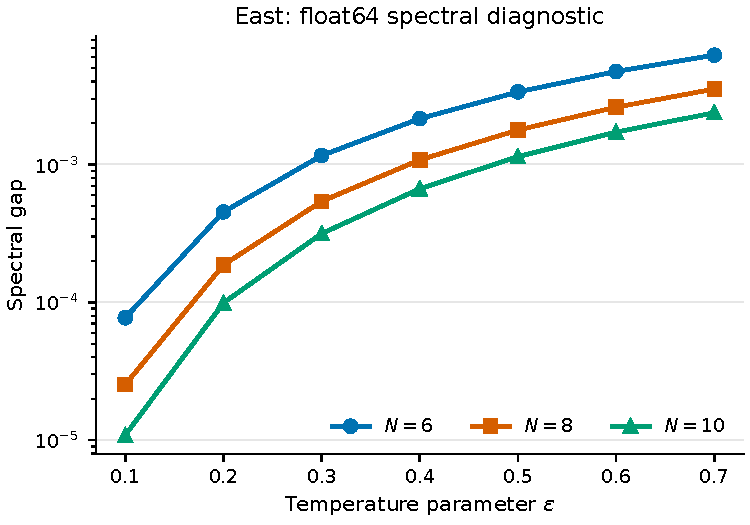
\includegraphics[width=0.7\linewidth]{figures/out/fig_spectral_gaps.pdf}
  \caption{East-model spectral gaps across the declared $(N,\epsilon)$ grid (float64 diagnostic
    used only for window calibration).}
  \label{fig:spectral-gaps}
\end{figure}

\section{GT1: The Energy Readout Is Not Closed}
\label{sec:gt1}
%% Packet W-03. Ledger rows: GT1, GB2, NEG.gt1_b_parity_control_open.

\subsection{Claim}

In plain terms: for an aging East chain, knowing the microstate tells you substantially more
about the energy a few steps ahead than knowing the present energy does, and it does so by a
certified factor more than at constrained equilibrium. The packaging defect of \S\ref{sec:methods}
is reported alongside as a second ratio. Precisely:

\claimref{GT1}{a0cea276116f05fcbb10844c527aac69d2027c70210a19db4753364d6c54d44e}
On the declared scope (East model, $N=8$, lens $L_{\mathrm{energy}}$, $\tau$ ladder
$[1,2,4,8]$, quench cell $\epsilon: 7/10 \to 1/10$ with waiting time $t_w = 20$), the closure
deficit $\mathrm{CD}_\tau$ of the aging protocol exceeds the constrained-East
stationary-equilibrium baseline at every declared cell by at least the declared margin $3/2$
(achieved minimum ratio $\approx 1.6392$; Table~\ref{tab:gt1-margins}), and the audited
idempotence-defect table exceeds its declared margin $2$ (achieved ratio $289/121$). Grade:
theorem (audited class); evidence type as declared in the artifact: deterministic float64 for the
CD grid and its margin, exact rational for the idempotence-defect ratio and the lumpability
controls. In the framework's filing vocabulary the claim reads: the P5 channel of the standard
thermodynamic packaging is not \texttt{active\_projection} as a closed packaging on this declared
glassy scope; that is, packaging the present energy readout does not yield a closed description.
Anchors: F-III T8, F-I D-IC-01/D-IC-02/T-CL-01, \sbtcite{sbt-paper-b} Def.~3.1.

\begin{longtable}{rrrr}
\caption{GT1 closure deficit vs. constrained-equilibrium baseline (East N=8, L\_energy)}\label{tab:gt1-margins} \\
\toprule
$\tau$ & $CD_\tau$ (glassy) & $CD_\tau$ (equilibrium) & ratio \\
\midrule
\endfirsthead
\toprule
$\tau$ & $CD_\tau$ (glassy) & $CD_\tau$ (equilibrium) & ratio \\
\midrule
\endhead
\bottomrule
\endfoot
1 & 0.033650 & 0.018875 & 1.7828 \\
2 & 0.063730 & 0.036068 & 1.7669 \\
4 & 0.113110 & 0.065575 & 1.7249 \\
8 & 0.177212 & 0.108112 & 1.6392 \\
\textbf{margin} & -- & -- & declared 3/2, achieved 1.6392 \\
\bottomrule
\end{longtable}


\subsection{The control structure, including a corrected expectation}

The controls deserve emphasis because one of them corrected our own design document. The design
called for constrained-East equilibrium to serve as a zero-deficit control, on the intuition that
an equilibrated chain has nothing left to remember. That intuition is \emph{false}, and provably
so. $\mathrm{CD}_\tau = 0$ if and only if the energy readout is $\tau$-lumpable, and
whether it is depends on the kinetic constraint, not on stationarity: in East a spin can
flip only when its left neighbor is up, so the number of spins free to move, and hence the rate
at which the energy can change, depends on \emph{where} the up spins sit, not merely on how many
there are. So the energy
readout of East is not closed even at equilibrium. The shipped certificate therefore uses two
controls with different jobs (Fig.~\ref{fig:gt1-ladder}): the \emph{unconstrained} model, whose
energy readout is lumpable by construction, sits at exact rational $\mathrm{CD} = 0$ (float
residuals at $10^{-17}$, exact lumpability verified symbolically), while constrained-East
equilibrium is an honest \emph{nonzero baseline}. The content of the certificate is that aging
exceeds even that baseline by the declared margin. Equilibrium is not used as a zero control
anywhere.

\claimref{GB2}{847f389464f9196f2315c05e3cef842efa94f201aad26f19b5dc4071e043f081}
Because the aging chain is driven by a temperature schedule, the closure deficit must be defined
relative to the protocol rather than to a single stationary kernel. The machinery for that is the
GB2 demo: finite protocol-relative CD computations (East versus unconstrained, $N=4$, declared
$\epsilon$ grid) with exactness reserved for the lumpability check and float64 windowed
diagnostics labeled as such. GB2 is recognition-grade, a demonstration rather than a certificate,
and the GT1 artifact carries a passing consistency gate for it: in the stationary limit the
protocol-relative deficit reproduces the stationary deficit with residual exactly $0$.

\begin{figure}[htbp]
  \centering
  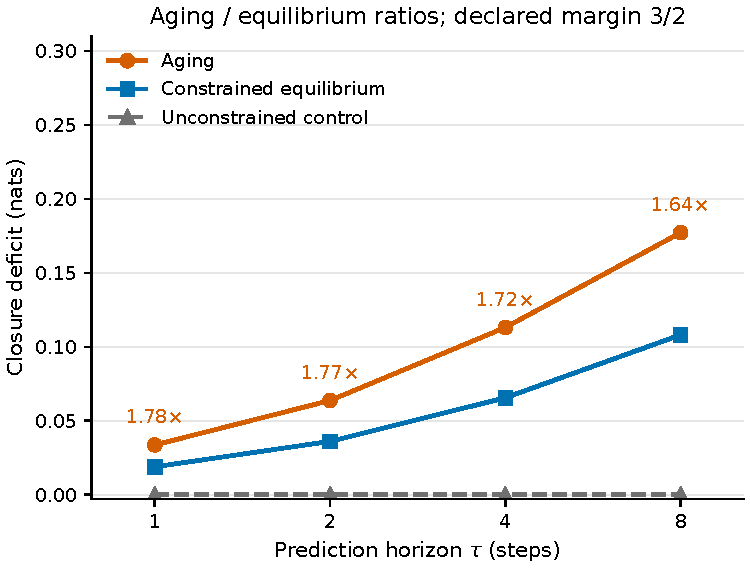
\includegraphics[width=0.7\linewidth]{figures/out/fig_gt1_cd_ladder.pdf}
  \caption{GT1 closure deficit (nats) versus horizon $\tau$: aging protocol, constrained-equilibrium
    baseline (nonzero because the energy readout is not lumpable), and the unconstrained control at
    exact zero. Annotations give the aging/equilibrium ratio at each horizon against the declared
    margin $3/2$.}
  \label{fig:gt1-ladder}
\end{figure}

\subsection{Scope and open control}

The certificate quantifies over exactly its declared cell: East, $N=8$, $L_{\mathrm{energy}}$,
the declared $\tau$ ladder and quench window. FA replication, the richer $L_{\mathrm{panel}}$
lens, and $N=10$ are extensions that were not run, listed as such in the artifact envelope.

\claimref{NEG.gt1\_b\_parity\_control\_open}{a0cea276116f05fcbb10844c527aac69d2027c70210a19db4753364d6c54d44e}
One intended control is open: the paper-[B] example-chain benchmark-parity check was not ported,
and the GT1 artifact files it as an explicitly skipped control with its reason
(machine-readable \texttt{status: skipped}). The certificate's margins are internal to its own
declared scope and do not route through [B]'s example chains; no [B]-parity is claimed until the
control is actually run.

\section{GT2 and GT5: The Kovacs Witness and What It Costs to Repair}
\label{sec:gt2-gt5}
%% Packet W-04. Ledger rows: GT2, GT5, NEG.gt2_loop_certificate_not_built.

\subsection{The Kovacs protocol on the audited class}

The Kovacs protocol \cite{kovacs-1963} (equilibrate hot, quench cold, age for $t_w$, jump up to
an intermediate temperature, watch a one-time observable relax) was located on the East substrate
by an exact search, run before any certificate and filed as a pre-certificate control. At $N=10$,
$\epsilon: 7/10 \to 1/10 \to 2/5$ with $t_w = 40$, the mean energy after the second jump starts
below its new equilibrium value $20/7 \approx 2.857$ (at $\approx 2.741$), crosses it between
steps $1$ and $2$ ($\approx 2.803$ and $\approx 2.859$), and overshoots through a hump peaking at
$t_{\mathrm{peak}} = 35$ before returning (Fig.~\ref{fig:kovacs-hump}), all in exact rational
arithmetic; $t_K = 1$ denotes the last step before the crossing. The raw trace never equals
$20/7$ at an integer step; the preparation that does, a randomized stop between steps $1$ and $2$,
is constructed in \S\ref{sec:gt2-witness}. The non-monotone excursion after the crossing is the
classic signature that the present value does not determine the future; for a finite Markov chain
in the linear-response regime, Prados and Brey showed it is generic whenever the observable's
relaxation is not a single exponential \cite{prados-brey-2010}. That East- and FA-type models show a Kovacs hump was established
numerically by \cite{buhot-2003,arenzon-sellitto-2004}; what is new here is the exact-rational
trace and the certificate built on it.

\begin{figure}[htbp]
  \centering
  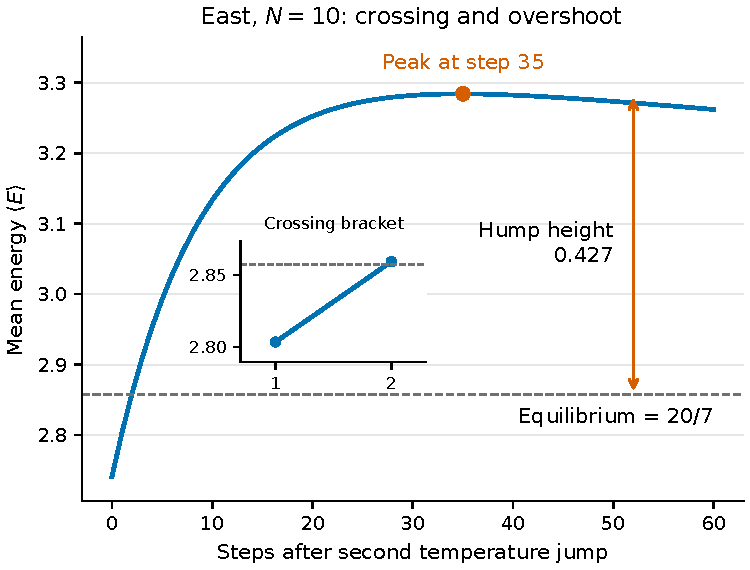
\includegraphics[width=0.7\linewidth]{figures/out/fig_gt2_kovacs_hump.pdf}
  \caption{Kovacs hump on East $N=10$ (exact-rational trace, floats only for plotting): the mean
    energy starts below its equilibrium value $20/7$, crosses it between steps $1$ and $2$
    (inset), peaks at step $35$, and returns toward equilibrium.}
  \label{fig:kovacs-hump}
\end{figure}

\subsection{GT2: the witness certificate}
\label{sec:gt2-witness}

In plain terms: we exhibit two preparation histories of the East chain with exactly the same
present mean energy and provably different mean energies five steps later. The first history is
the Kovacs run stopped at the crossing: since no single time step lands exactly on $20/7$, the
run is stopped at step $1$ with probability $\theta \approx 0.0359$ and at step $2$ otherwise,
with $\theta$ solved exactly so that the mixture's mean energy is $20/7$ (a ``randomized stop'',
a declared move of the pipeline). The second history is the equilibrium distribution at
$\epsilon = 2/5$, whose mean energy is $20/7$ by definition. Both are then held at
$\epsilon = 2/5$ for five steps and their mean energies compared: the equilibrium history stays
at $20/7 \approx 2.857$ while the Kovacs history has moved to $\approx 3.058$, a gap of
$\approx 0.201$. Only the mean energy is matched at the start, not the full energy distribution;
that is exactly what the energy readout, as a lens, sees. Precisely:

\claimref{GT2}{321f9bffdbf1368ec764a8fcde97d569dd9f4292ee5a98a0b6f30ac9483ce7bf}
On the declared scope (East, $N=10$, \texttt{kovacs\_moment} lens, declared $\epsilon$ grid and
continuation catalog), one exact-rational split pair of preparation histories is exhibited: the
two histories agree on the present lens value (mean energy $20/7$) and their futures differ, with
an exact maximum absolute future gap that is a strictly positive rational number
($\approx 0.2005$ on the five-step hold; the exact fraction is in the artifact). By
\sbtcite{sbt-paper-a} Thm.~3.5, the existence of such a pair is equivalent to the comparison map
$\pi: M \to Q$ being strictly refining, that is, to the predictive description being genuinely
finer than the present-observable one. Grade: theorem (audited class).

The framework distinguishes three things a ``different future'' could mean, and we claim only the
first: that the future depends on more than the present readout; \emph{not} that the two
histories took different routes to the same state (a P3 route mismatch); and \emph{not} any
directionality or irreversibility. In the framework's filing vocabulary the first reading is
\textbf{P4 staged-dependence}, filed on the standard witness template (F-II
\texttt{prop:p1-witness}). No P6\_drive audit was performed, so no arrow-of-time statement of any kind is
made on GT2's behalf.

\claimref{NEG.gt2\_loop\_certificate\_not\_built}{321f9bffdbf1368ec764a8fcde97d569dd9f4292ee5a98a0b6f30ac9483ce7bf}
The proposal also called for a companion certificate about thermal loops (a closed temperature
cycle acting trivially on the present description $Q$ but nontrivially on the predictive
description $M$). It was not built: the split-pair witness stands alone, and, as
\S\ref{sec:lean} makes precise, the vendored formal core cannot even express a non-vacuous
loop-asymmetry instance, so a computational loop certificate would first need new formal footing.
Disclosed here and in the gap register; nothing downstream depends on it.

\subsection{GT5: what it costs to buy the distinction back}

In plain terms: adding a single scalar to the energy readout is enough to tell the two witness
histories apart, and a fictive-temperature-like index is one of three declared choices that
work. Precisely:

\claimref{GT5}{746b44e6c2f7f92364137a202f7306b6afc9e99c413fb4dd3a40d47bfd6f94c8}
On the declared scope (East, $N=10$, \texttt{kovacs\_moment} interface, the declared two-history
class), the present lens collapses the witness pair into one class ($|Q| = 1$ on the pair) while
the predictive quotient keeps two ($|M| = 2$), so the largest fiber of $\pi$ has size
$\mathrm{MaxFiber} = 2$, meeting the nontriviality threshold. The buyback curve
(Fig.~\ref{fig:buyback}) is published as a lift ledger per F-II \texttt{prop:forgetting-lifts}:
each added memory coordinate is a recorded, selected, non-unique lift. At budget $0$ the pair is
unresolved; at budget $1$, \emph{each} of the three declared scalar coordinates already resolves
it exactly (loss $0/1$), so the shipped witness saturates at $\texttt{saturation\_budget} = 1$.
The three coordinates are expectations over the history's microstate distribution $\mu$ of a
per-microstate quantity: $T_f(\mu) = \mathbb{E}_\mu[\,i^*(E(n))\,]$, where $i^*(E)$ is the
index of the grid value $\epsilon_i$ whose equilibrium mean energy is closest to $E$ (an index
into the declared grid, not a temperature, and not inferred from the history's mean energy, so
two histories with equal mean energy can have different $T_f$); $D(\mu)$, the expected number
of adjacent up-up spin pairs; and $n_1(\mu)$, the expected occupation of the site next to the
wall.

The translation to the glass literature is deliberately modest. The TNM fictive temperature
\cite{tool-1946,narayanaswamy-1971,moynihan-1976,hodge-1994} is the motivating analogy for $T_f$: an
energy-indexed effective temperature added as a declared step from the present description
toward the predictive one. The implemented $T_f$ is the grid-index construction above, not the
TNM quantity itself. Modern treatments of the Kovacs effect likewise pair an effective
temperature with a second structural variable \cite{bouchbinder-langer-2010}, and the
multiparameter models the Kovacs literature moved to \cite{kahr-1979} are why the general
insufficiency question is left open here rather than answered on one pair. For
\emph{this} minimal two-history witness, one scalar suffices; the certificate demonstrates the
repair \emph{mechanism} and its ledger discipline. It is not a claim that a single
fictive-temperature-like scalar is insufficient in general: such a claim would require a richer
multi-instance construction that was not built here.

\begin{figure}[htbp]
  \centering
  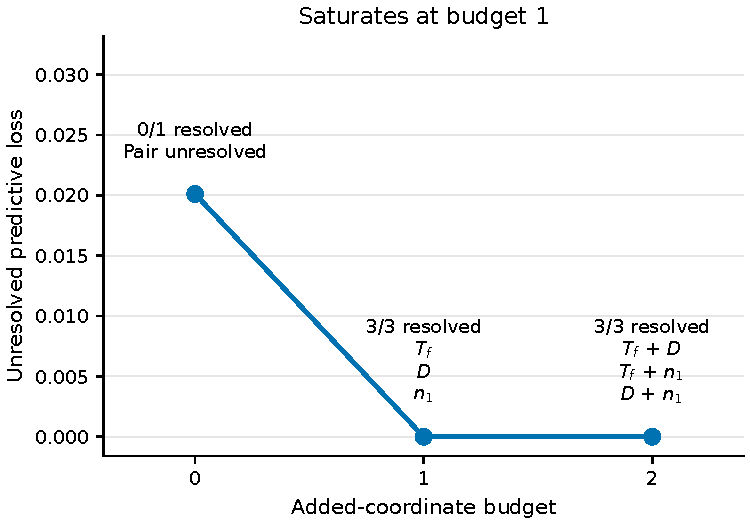
\includegraphics[width=0.7\linewidth]{figures/out/fig_gt5_buyback.pdf}
  \caption{GT5 buyback curve: unresolved predictive loss versus added-coordinate budget, annotated
    with resolved/attempted counts and the resolving coordinates. The loss is the budget envelope
    of the two-point squared prediction error $(a-b)^2/2$, where $a$ and $b$ are the two
    histories' five-step future mean energies, incurred only while the pair is left in one class
    ($\approx 0.0201$ at budget $0$, i.e.\ half the squared witness gap); a group that separates
    the pair has loss $0$. The shipped two-history witness saturates at budget $1$.}
  \label{fig:buyback}
\end{figure}

\section{GT3 and GT4: Foreclosure and the Kill-Test Panel}
\label{sec:gt3-gt4}
%% Packet W-05. Ledger rows: GT3, GT4, GB1.

\subsection{GT3: the order-parameter search, foreclosed on its declared class}

In plain terms: a static order parameter built from the energy readout is a function of the
energy value. On $N=8$ spins the energy takes $9$ values, so there are exactly $2^9 = 512$
yes/no functions of it, and we can check them all. Every one of them agrees on a pair of histories
that a finer readout of the same microstate, the occupation of the site next to the wall, tells
apart. Precisely:

\claimref{GT3}{25e78910189098978f58f5e083cd3553f42fd9eb2b94cc7818d0ed80f0f661a7}
On the declared scope (East, $N=8$, $\epsilon = 1/2$), the definability bound of F-III T14 makes
the static-order-parameter search space finite: a fixed lens with image size $9$ defines exactly
$2^9 = 512$ predicates. The sweep checks all $512$: every one agrees on the exhibited witness
pair, while a distinguishing readout based on $n_1$ (the occupation of the site next to the wall)
separates it, with exact gap $169/1536$ on the separating continuation
(Table~\ref{tab:gt3-foreclosure}). The witness pair is a standalone reflection pair
constructed for this sweep, deliberately \emph{not} chained to the GT2 certificate, so the two
results fail independently. This is a constructive foreclosure: the distinguishing readout is
exhibited and proven absent from the set of energy-definable predicates, not inferred from
counting. Grade: theorem (audited class).

\begin{longtable}{lp{9cm}}
\caption{GT3 foreclosure sweep summary (East N=8, $\epsilon=1/2$)}\label{tab:gt3-foreclosure} \\
\toprule
field & value \\
\midrule
\endfirsthead
\toprule
field & value \\
\midrule
\endhead
\bottomrule
\endfoot
N & 8 \\
epsilon & 1/2 \\
lens & L\_energy \\
total predicates & 512 \\
agreeing predicates & 512 \\
lens image size & 9 \\
all agree & True \\
separating event & n\_1 \\
witness provenance & standalone W\_reflection witness constructed for this sweep; not chained to the GT2.kovacs\_moment certificate (a separate witness family per design/specs/04\_gt2\_witnesses.md §4). \\
T-FOR-02 statement & the distinguishing readout (n\_1-based) is not in Def(l\_energy); constructive witness exhibited, not generic counting \\
\bottomrule
\end{longtable}


The field-facing sentence, ``there is no static order parameter for glass,'' is licensed here
\emph{only} as the declared-class shadow of this theorem (F-II item E2), with the class, the
catalog, and the suppressed content named in the same breath: no predicate definable from the
declared energy lens on the declared class separates what memory separates. Reading it as a
statement about other instruments, other lens classes (in particular the amorphous order of
random first-order transition theory \cite{kirkpatrick-thirumalai-wolynes-1989,lubchenko-wolynes-2007},
the configurational-entropy line descending from \cite{adam-gibbs-1965}, or the local-structure
measures surveyed in \cite{royall-williams-2015}), or the continuum is not licensed, and this
paper does not do so. What the theorem does license, via the framework's no-free-distinction law
(F-IV F12), is narrower and exact: any readout that \emph{does} separate this pair must carry
declared information beyond the energy readout. Here that information is a present structural
coordinate of the microstate ($n_1$, under the identity continuation), not a record of the
history; the separation shows that the energy-based description is incomplete, and GT5
separately shows that one added coordinate, structural or history-based, suffices to repair it
on the Kovacs pair.

\subsection{GT4: the kill-test panel}

A memory signature can be faked. GT4 builds five schematic fixtures for the ways it can be
faked, each a small package of two or three microstates at $N=4$ with declared readouts and
continuations, and checks that the same deterministic classifier that accepts the Kovacs
candidate (a reflection pair at $N=8$, distinguishable by the full spin panel but not by its
reflection-invariant part) rejects all five. The fixtures are regime schemata, not physical
mechanisms: the ``protocol trap'' pair carries a residue of its schedule in the readout, and its
``honest'' twin replaces the identity continuation by a constant reset so the residue is no
longer future-visible; the ``flattenable'' pair does the same for an incomplete continuation
catalog; the ``explicitly latent'' pair differs in a bit the present readout does not see; the
``dissipative'' fixture merges the two histories at a later interface; and the ``flat'' control
is two copies of the $N=4$ equilibrium distribution, which by construction has nothing to
separate. Precisely:

\claimref{GT4}{160ed9c4bb65a8189f012fba1fb7e4a55fc17e323050437206c341c077b53619}
Over the declared $9$-member thermal benchmark family, the deterministic triage classification
identifies \texttt{kovacs\_wheel}, the Kovacs memory candidate, as the sole
\texttt{coherent\_candidate}, while the five declared non-coherent regime controls
(\texttt{artifact\_trap}, \texttt{dissipative}, \texttt{explicit\_latent}, \texttt{flat},
\texttt{flattenable}) are correctly killed or cleared (Table~\ref{tab:gt4-regime-triage}).
Protocol-trap discipline is applied: raw and cleared classifications are both recorded, so the
table shows each artifact being caught (for instance, the naive protocol-trap fixture classifies as \texttt{artifact\_trap} raw and
its constant-reset twin as \texttt{flat}). Grade: theorem (audited class), over the declared finite family only, not a
shell-general theorem.

\begin{longtable}{lll}
\caption{GT4 regime triage over the declared benchmark family}\label{tab:gt4-regime-triage} \\
\toprule
regime & raw classification & cleared classification \\
\midrule
\endfirsthead
\toprule
regime & raw classification & cleared classification \\
\midrule
\endhead
\bottomrule
\endfoot
coherent candidate & kovacs\_wheel & -- \\
artifact\_trap & protocol\_trap\_naive & protocol\_trap\_honest \\
dissipative & dissipative\_memory@mid & dissipative\_memory@end \\
explicit\_latent & latent\_memory\_base & latent\_memory\_refined \\
flat & flat\_control & (pure control, no repair) \\
flattenable & flattenable\_raw & flattenable\_completed \\
\bottomrule
\end{longtable}


\subsection{GB1: the protocol-trap caveat, carried openly}

The ``protocol trap'' is a warning about arrows of time, not about memory: a system whose
dynamics switch between several kernels under a clock can show a spurious time asymmetry if the
clock is left outside the state. The framework's published theorem on this (F-I T-AOT-02) says
that when the clock is reversible and every phase kernel is reversible with respect to a
\emph{common} stationary measure, the autonomous lift of the system has zero entropy production
and zero path-reversal asymmetry at every horizon, so any observed arrow must come from an
external schedule or a stroboscopic fit. Kovacs kernels $K_\epsilon$ are reversible with respect
to different Gibbs measures for each $\epsilon$, so the theorem does not apply as published, and
the temperature switches contribute a nonzero boundary term.

\claimref{GB1}{4173705a52c358bc74b51815929cb2a28c8f680b3421dafdb7633e97b051fa8e}
GB1, the temperature-protocol version in the style of the protocol-trap microarticle
\sbtcite{sbt-protocol-trap}, ships as a recognition-grade mathematical demonstration: an exact
identity for that boundary term (a pseudo-entropy-production identity) plus a finite exact
numerical check, with the general inequality filed as an explicitly open obligation in the
artifact payload. Its role is to keep the arrow-of-time audit separate from the memory
classification: GT4's triage computation is deterministic and exact, but the clock-audit
\emph{discipline} it applies (raw versus cleared classification) rests, for temperature
protocols, partly on this demonstration rather than on a closed theorem. This is the framework's
conditional-reporting rule working as designed.

\section{GT6: The Memory Layer Strictly Extends the Observable Layer}
\label{sec:gt6}
%% Packet W-06. Ledger rows: GT6, NEG.material_forcing_absent.

\subsection{Claim and verdict basis}

In plain terms: describing an East glass by the future-equivalence class of its preparation
history carries information that the declared energy-based description cannot, and the
framework's checklist for certifying such a statement (a gate table with pass/fail rows, plus
ablations) is completed for the audited shell, the frozen eligibility conditions defined in
\S\ref{sec:methods}. Precisely:

\claimref{GT6}{6453d0e36a5f43e0a3e7ed9f69f53e00a3c6cef7aa1ddea4019522d5670cab97}
For the audited East glass shell ($N=8$, declared $\epsilon$ grid and protocol windows), the
promotion filing of F-III \S10 (bridge record, gate table, knockout panel, nonclaim register,
checker) is complete, and the gate-table verdict is \texttt{strict}: the predictive-structure
layer strictly extends the current-observable layer on this shell. Grade: certificate
(shell-local, the standard of paper [C] \sbtcite{sbt-paper-c}): valid on the frozen shell, with
no broader-class transfer claimed.

Because an earlier draft of this project's own design documents overstated this result, the basis
of the verdict is quoted verbatim from the audit artifact rather than paraphrased:

\begin{quote}
``verdict: strict is established via F-III T19/T20 (non-factorization from GT2/GT3 witnesses).
Paper [C]'s thm:strict-extension (the fuller completion-dynamics route requiring material
P4$\leftarrow$P5 forcing) is NOT invoked: H4\_forcing.material\_forcing\_count = 0 for this shell,
filed as an honest negative sub-result, not as a satisfied hypothesis.''
\end{quote}

That is: the strictness verdict rests on \emph{non-factorization}. GT2 exhibits histories that
the energy-based description merges and the predictive one separates, and GT3 shows that no
energy-definable predicate can undo the merge, so the predictive description cannot be a function
of the energy-based one; the framework's theorems T19/T20 turn that into the verdict. The verdict does
\emph{not} rest on paper [C]'s stronger completion-dynamics theorem, whose ``material forcing''
hypothesis this shell simply does not satisfy. (Material forcing means that the catalog of
protocols contains \emph{conditioned} schedules, in which the next temperature step depends on
the measured panel, as in real glass processing, and that some distinctions between histories
exist only because of them. The audited catalog produced none.)

\claimref{NEG.material\_forcing\_absent}{f5f9558e0ffa786ac8a28254e555d398eff572d2936aea89a889ea160cb7bed2}
The forcing check itself is a result: $\texttt{material\_forcing\_count} = 0$ on the audited
shell. Absence of material forcing here is not evidence about other shells or protocols; it marks
the exact boundary of which [C] machinery this instantiation exercises.

\subsection{Gate table and knockout panel}

The gate table (Table~\ref{tab:gt6-gate-table}) lists the framework's required checks for a
strict-extension verdict and the evidence for each; two rows are marked not required because the
claim is about enrichment of the description, not about a closed macroscopic dynamics.

\begin{longtable}{lllp{6.5cm}}
\caption{GT6 gate table (audited glass shell)}\label{tab:gt6-gate-table} \\
\toprule
gate & required & status & evidence \\
\midrule
\endfirsthead
\toprule
gate & required & status & evidence \\
\midrule
\endhead
\bottomrule
\endfoot
G\_suff & True & pass & audit.json filing assembled \\
G\_desc & False & not\_required & glass bridge claims strict object-map enrichment, not closed macro dynamics \\
G\_stab & True & pass & P3-04 saturated strata under E\_{tau,f} \\
G\_ctrl & True & pass & P3-01 knockout panel controls \\
G\_nosmuggle & True & pass & six no-smuggling violation kinds checked \\
G\_vis & True & pass & visible citations and nonclaims filed \\
G\_audit & True & pass & checker validates hashes and verdict \\
G\_strict & True & strict\_pass & GT2/GT3 constructive split witnesses \\
G\_locglob & False & not\_required & shell-bound single bridge only; no stacked or glued promotions claimed \\
\bottomrule
\end{longtable}


The knockout panel (Table~\ref{tab:gt6-knockouts}) is an ablation study: each of the six
primitives P1--P6 that the framework says a closed description can depend on is disabled in turn,
and the effect on the result is recorded, in two distinct modes that the artifact's own nonclaim
keeps separate. For P1--P3 the knockouts are \emph{numeric}: disabling the primitive (identity
run kernels; the unconstrained-lumpable replacement; constant-$\epsilon$ replacement) degrades a
declared numeric diagnostic past its declared threshold. For P4--P6 the knockouts are
\emph{capability-loss} rows: removing the primitive makes the relevant downstream diagnostic
unavailable or undefined rather than numerically degraded. There is no numeric threshold to cross
in those rows, and none is claimed.

\begin{longtable}{lllp{6.5cm}}
\caption{GT6 knockout panel}\label{tab:gt6-knockouts} \\
\toprule
primitive & kind & degraded & threshold \\
\midrule
\endfirsthead
\toprule
primitive & kind & degraded & threshold \\
\midrule
\endhead
\bottomrule
\endfoot
P1 & numeric & True & identity trace variation must be exactly 0 \\
P2 & numeric & True & unconstrained control must be exactly lumpable under L\_energy \\
P3 & numeric & True & constant-epsilon replacement must fail the hump detector \\
P4 & capability\_loss & True & -- \\
P5 & capability\_loss & True & -- \\
P6 & capability\_loss & True & -- \\
\bottomrule
\end{longtable}


Supporting diagnostics are filed at their true, lower grades: the Fekete pressure-closure table is
a float64 diagnostic (not an exact-rational certificate; sparse $N=10$ rows skipped by declared
threshold and reported as such), and the spectral-gap table (\S\ref{sec:models}) calibrates the
shell windows only. The gate row H5 (the macro-admissibility obstruction) cites the GT1
theorem-grade certificate by content hash; paper [C] itself glosses this obligation as failure of
admissible aggregation or lumpability at the macro level, which is precisely what GT1 certifies.

\subsection{What strictness does not mean}

The artifact's nonclaim register (printed in full in \S\ref{sec:discussion}) is part of the
result. In particular: strictness is shell-local (no shell-general strict-bridge theorem, no
broader-class transfer); strictness does not imply that the memory layer has an autonomous closed
dynamics of its own, nor that anything drives it (no P6\_drive audit was performed); the pressure
gap is neither a closure deficit nor the strictness witness; and the promotion is a single bridge
$T_0 \to T_1$. The framework has no theorem for stacking such bridges, and none is used.

\section{GT7: Aging Constants Are Run-Only: Freeze, Transfer, and the Scoreboard}
\label{sec:gt7}
%% Packet W-07. Ledger rows: GT7, NEG.gt7_transfer_failures.

\subsection{The protocol}

GT7 asks whether the numbers that characterize aging on East (Kovacs crossing time, peak time,
hump height, and three others) carry over to a different model without any fitting. The answer
was obtained the way a pre-registered experiment is \cite{nosek-et-al-2018,munafo-et-al-2017}: the readouts were fixed, the East reference
was computed, predictions for the target models were committed and hashed, and only then were the
targets run and scored by a script that had itself been frozen. Precisely:

\claimref{GT7}{4905b013624462549b9a4cdb18f51d0220f70be29976be461e5a8681978dcab8}
GT7's claim is a discipline plus its unedited outcome. The freeze-and-transfer protocol ran in
five stages, each frozen by sha256 content hash before the next began:

\begin{itemize}
  \item \textbf{F1, readouts freeze.} Six declared readouts (Kovacs $t_K$, $t_{\mathrm{peak}}$,
    hump height, memory-dimension profile, deficit-decay slope, cross-validation checks) frozen in
    a registry with content hash and freeze note.
  \item \textbf{F2, East reference.} The reference surface on East: 56 exact hump-surface cells
    at $N=10$, an $N=16$ Monte Carlo spot check, the closure-deficit ladder (Fig.~\ref{fig:deficit-decay}) whose declared secant slope is the
    frozen deficit-decay readout, and memory-dimension profiles. Run-only readouts; no functional form fitted anywhere.
  \item \textbf{F3, pre-registration.} 338 predictions committed before any target-family run:
    42 interval predictions, 2 order-relation predictions, and 294 cells explicitly declared
    \texttt{no\_prediction}. The predictions registry pins the frozen readouts hash, the East
    reference hash, and the hash of the scoring script itself.
  \item \textbf{F4, target runs.} FA and trap families run blind against the committed
    predictions.
  \item \textbf{F5, mechanical scoring.} The frozen scorer (hash-pinned at F3, verified
    unchanged) compares predictions to observations with no post-hoc widening or
    reinterpretation.
\end{itemize}

\begin{figure}[htbp]
  \centering
  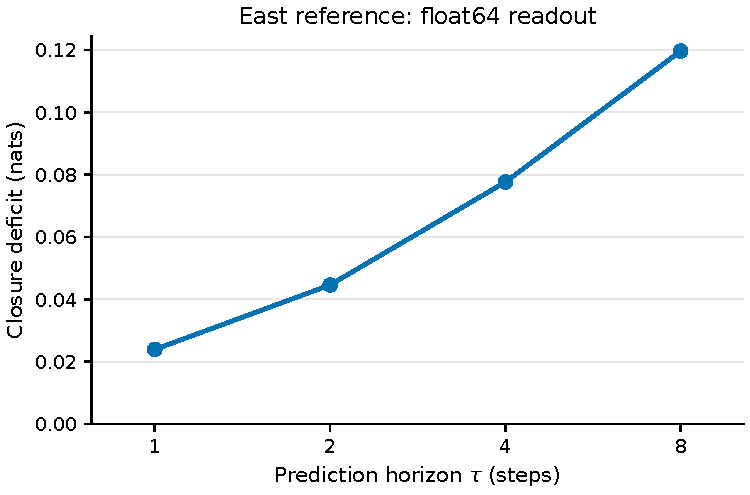
\includegraphics[width=0.7\linewidth]{figures/out/fig_gt7_deficit_decay.pdf}
  \caption{East-reference closure deficit (nats) across the declared $\tau$ ladder (run-only
    float64 readout; part of the frozen F2 reference). The frozen ``deficit-decay'' readout is the
    declared secant slope between two ladder points, not a fit; the deficit itself grows with
    horizon.}
  \label{fig:deficit-decay}
\end{figure}

\subsection{The scoreboard, unedited}

\claimref{NEG.gt7\_transfer\_failures}{37ac2b8f4bcb55cf1f2cf9f0518850a84039c3e51177d3000d0244b5ed6cc96e}
Of the 44 committed predictions, 22 were scored against observed target cells: \textbf{8 passed
and 14 failed}; the other 22 targeted cells that produced no observation. All 338 verdicts are
filed unedited (Fig.~\ref{fig:scoreboard}). The failure pattern is itself a filed, tested fact:

\begin{itemize}
  \item All 14 failures are FA-family interval predictions (5 $t_K$, 4 $t_{\mathrm{peak}}$,
    5 hump-height), and every one is \emph{one-sided high}: the observed FA value exceeds the
    predicted upper bound. FA humps are systematically later and larger than the East-anchored
    intervals allowed.
  \item Failures cluster at the deeper intermediate temperature: 12 of 14 failing cells have
    $\epsilon_{\mathrm{mid}} = 2/5$, where every scored cell failed. At
    $\epsilon_{\mathrm{mid}} = 1/2$, 7 of 9 scored interval cells passed (plus the passing
    order-relation prediction), and the two misses there are borderline (hump height $0.2033$
    against a bound of $0.2008$; $t_K$ of $5$ against $[1,3]$).
  \item All 22 unobserved cells are trap-family: the trap target's exact hump search returned
    \texttt{found = false} in all 56 surface cells, with the uniform miss reason ``does not start
    below equilibrium.'' This is the dynamical corollary of the $\epsilon$-invariance lemma of
    \S\ref{sec:models}: since the declared trap family's equilibrium does not move with
    $\epsilon$, a temperature jump never leaves it below its new equilibrium, and the Kovacs
    protocol cannot produce a hump there at all.
\end{itemize}

\begin{figure}[htbp]
  \centering
  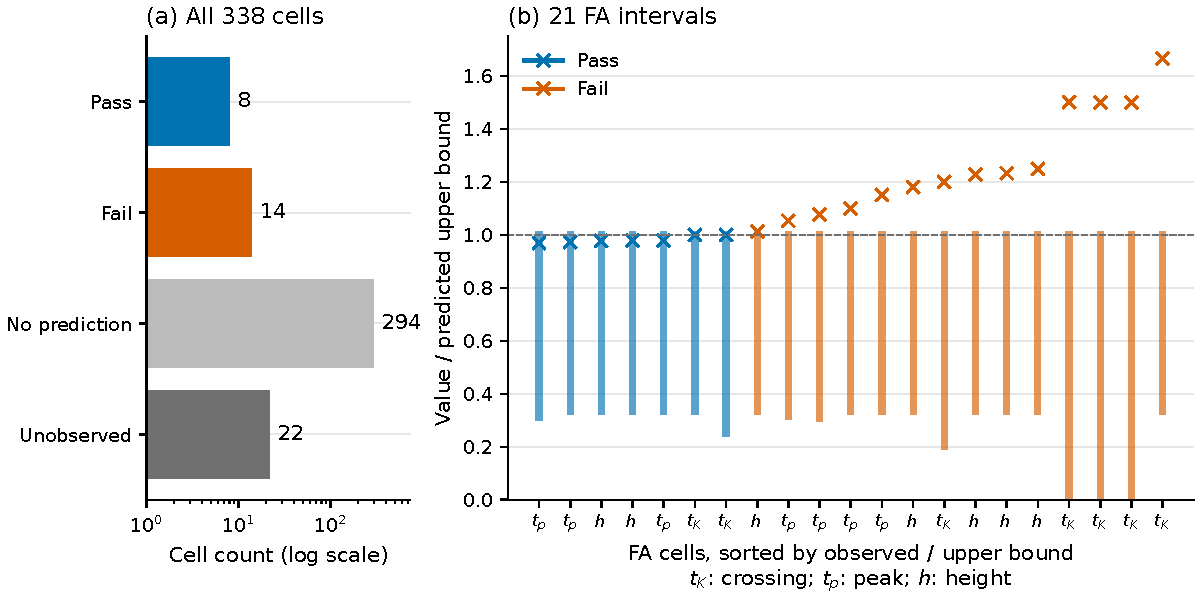
\includegraphics[width=\linewidth]{figures/out/fig_gt7_transfer_scoreboard.pdf}
  \caption{Left: verdict counts over all 338 cells (log scale). Right: the 21 scored FA interval cells
    (the 22nd scored FA prediction is the order relation, not plotted); each interval and its
    observed value are divided by the interval's upper bound, and cells are sorted by that ratio,
    so every failure lies above the dashed line at $1$.}
  \label{fig:scoreboard}
\end{figure}

\subsection{Reading the failures}

The failures are first-class results of the pre-registration protocol: it is designed to be
falsifiable, and it was. Three readings are compatible with the data, and the protocol forbids
choosing among them after the fact: (a) East-to-FA transfer of run-only constants degrades with
quench depth, in the direction of FA responding slower and larger; (b) the declared rule for
scaling East intervals to FA, rather than the readouts themselves, is what failed; (c) the trap
column is not a partial failure but a structural mismatch between the protocol and the declared
trap family, predicted in hindsight by the $\epsilon$-invariance lemma. Under any reading, the
run-only thesis stands as filed: the readouts are readouts of runs, frozen, transferred, and
scored, not fitted. (GT3's non-definability result concerns its own witness pair and the energy
lens; it is not extended here to the GT7 readouts, for which no such witness was constructed.) Score counts are not a fitted scaling law, and no post-hoc reinterpretation of failed
intervals is permitted or performed.

\section{GB9: The Lean-Checked Core and the Scope-Boundary Finding}
\label{sec:lean}
%% Packet W-08. Ledger rows: GB9, FINDING.lean_collapse, NEG.lean_instance_structural.

\subsection{What is machine-checked}

Lean \cite{de-moura-ullrich-2021} is a proof assistant: a theorem stated in it is accepted only when a machine has checked
every step, and a development ``compiles sorry-free'' when no step has been left as an
unproved placeholder. We use it for the abstract theorems the certificates rely on (for example,
that a witness pair exists if and only if the predictive description is strictly finer than the
present one), so that those steps do not depend on a reader trusting the prose. Precisely:

\claimref{GB9}{014c387c154a27d21d86e0454c25fea4ddc7ac8ecd3e7d3ea116d6f068a296c1}
The vendored \texttt{HolonomyMemory} core (paper [A]'s Lean development
\sbtcite{sbt-paper-a}) plus this project's \texttt{GlassWitness} extension compile sorry-free on
the pinned toolchain (\texttt{leanprover/lean4:4.29.0}), with per-theorem axiom audits. Per the
framework's fidelity legend, every row of the canonical 17-row fidelity table
(Table~\ref{tab:lean-fidelity-full}) carries its true label: 11 rows \emph{verified} (including
the three generic collapse theorems below and [A]'s witness/strict-refinement equivalence), 3
\emph{narrowed/parametric} (core structure fields), 1 \emph{typed mirror} (the glass instance), 1
\emph{schema projection}, and 1 \emph{computational evidence only} (the numeric Kovacs witness,
which is deliberately not encoded; see below). No schema or trivial declaration is described as a
verified proof anywhere in this paper, and closure-deficit computations are deterministic
computational evidence, not Lean theorems.

\begin{longtable}{lp{6cm}}
\caption{GB9 Lean fidelity table (all rows, printed in full per the Phase 5 gate; rows with no Lean encoding are labeled by the claim they document instead of a Lean identifier)}\label{tab:lean-fidelity-full} \\
\toprule
Lean name / documented claim & fidelity \\
\midrule
\endfirsthead
\toprule
Lean name / documented claim & fidelity \\
\midrule
\endhead
\bottomrule
\endfoot
futurePredictiveEquiv\_implies\_currentEventEquiv & verified \\
predictiveToCurrent\_commutes\_with\_transport & verified \\
predictiveQuotient\_futureSufficient & verified \\
futureSufficient\_stateEq\_implies\_futurePredictiveEquiv & verified \\
futureSufficient\_factorsThroughPredictiveQuotient\_onReachable & verified \\
futureSufficient\_factorization\_unique\_onReachable & verified \\
strictRefinement\_iff\_nonempty\_predictiveWitness & verified \\
loopAsymmetry\_exhibits\_movedPredictive\_fixedCurrent & verified \\
current\_implies\_future\_GENERIC & verified \\
predictiveWitness\_impossible\_GENERIC & verified \\
strictRefinement\_impossible\_GENERIC & verified \\
push\_id & narrowed / parametric \\
observe\_push & narrowed / parametric \\
push\_compose & narrowed / parametric \\
glassInstance & typed mirror \\
glassPredictiveQuotient\_futureSufficient & schema (projection) \\
Real Kovacs exact-rational numeric split-pair witness & computational evidence only \\
\bottomrule
\end{longtable}


\subsection{The collapse finding}

We intended to encode the numeric Kovacs witness of \S\ref{sec:gt2-gt5} in the core as well. The
attempt produced a theorem instead: in this core, no such witness can exist. Precisely:

\claimref{FINDING.lean\_collapse}{c70185334829fe8ad9f879a2288e90efe3d24700b8eeb5593f2de05341b62a51}
For \emph{every} instance of \texttt{RouteTransportCore}, the \texttt{observe\_push} coherence
field, combined with \texttt{CurrentEventEquiv}'s universal quantification over events, forces
current equivalence to imply future-predictive equivalence
(\texttt{current\_implies\_future\_GENERIC}); consequently non-vacuous \texttt{PredictiveWitness},
\texttt{StrictRefinement}, and \texttt{LoopAsymmetry} instances cannot be constructed in this core
at all (\texttt{predictiveWitness\_impossible\_GENERIC} and its strict-refinement companion;
machine-checked, sorry-free). The mechanism: the core's naturality axiom lets every future event
be pulled back to a present event, so ``agreement on all present events'' silently includes
agreement on all pulled-back futures, and there is nothing left for a witness to separate.

This is a genuine result about the formal core's expressiveness, strictly stronger than paper
[A]'s own declared boundary, and it has a familiar shape. It is the proof pattern of strong
lumpability for Markov chains \cite{kemeny-snell-1960,buchholz-1994}, where a local one-step
coherence condition propagates an equivalence to all future times; and it has the form of
biextensional collapse in the Chu-space sense \cite{barr-1979,pratt-1999,parente-2024}, with
\texttt{pullEvent} playing a role analogous to the Chu transform's naturality condition. We
offer the Chu-space reading as an analogy; no formal correspondence is claimed or proved here. The instructive
contrast is the causal-state construction of computational mechanics
\cite{shalizi-crutchfield-2001}, where agreement on the present generally does \emph{not} imply
agreement on the future: the collapse here is forced by this core's axiom, not a generic feature
of prediction.

\subsection{The consequence, stated as understanding rather than apology}

\claimref{NEG.lean\_instance\_structural}{014c387c154a27d21d86e0454c25fea4ddc7ac8ecd3e7d3ea116d6f068a296c1}
The finding explains exactly which certificates can live in Lean and which cannot. The abstract
theorems (witness if and only if strict refinement; factorization through $M$ and its uniqueness
on the reachable image) are verified generically and apply to any instantiation. But a
non-vacuous \emph{numeric} witness instance is unbuildable in this core, so \texttt{glassInstance}
is filed as what it is: a typed, index-based structural mirror, with the real Kovacs split pair
remaining exact-rational computational evidence in its own artifact (\S\ref{sec:gt2-gt5}). The
Python certificates avoid the collapse because they quantify over a finite \emph{declared} catalog
of futures rather than over all pullback-closed events. A formal core admitting numeric glass
witnesses would need weaker coherence axioms; that is future formalization work, now with a
machine-checked specification of exactly what must change.

\section{GB10: Empirical Bridge Records}
\label{sec:bridges}
%% Packet W-09. Ledger rows: GB10.

Nothing in the preceding sections is a measurement. The connection to the laboratory is made
through three \emph{bridge records}, drawn from the memory-effect phenomenology reviewed in
\cite{keim-2019}, each of which states what a real instrument sees, what it
suppresses, and under what threshold a measured signature would count as the laboratory
counterpart of one of our certificates. Precisely:

\claimref{GB10}{8015ce419a3a00e8a1b81217d0796ef53a6467db81cb774d0fa9711694087ab8}
Three empirical bridge records connect the formal complex to laboratory phenomena, each filed with
the complete five-field schema of F-II \texttt{prop:empirical-bridge} and validated by the bridge
checker: (i) \textbf{Kovacs PVAc volume recovery}
\cite{kovacs-1963,struik-1978,simon-sobieski-plazek-2001,bernazzani-simon-2002}, dilatometric
specific-volume measurement under the temperature-jump/age/second-jump protocol, with the level
map tying the measured hump to the GT2 witness artifact by content hash; (ii)
\textbf{spin-glass memory and rejuvenation}
\cite{jonason-et-al-1998,bouchaud-dupuis-hammann-vincent-2001,vincent-2007}; (iii) \textbf{colloidal-glass aging}
\cite{weeks-et-al-2000,courtland-weeks-2003,cipelletti-ramos-2005,peng-mckenna-2016}. Each record
carries: substrate and observable; instrument with a per-instrument visibility record (what the
apparatus sees and what it suppresses; dilatometry, for instance, sees one-time specific volume
and hump shape while suppressing the chain-conformation microstate); a level map with
formal-artifact hashes; a threshold--witness relation stating when a measured signature
\emph{counts} as a laboratory-grade witness; and suppressed-structure nonclaims.

The bridges are the paper's only channel to the laboratory, and they are deliberately one-way:
a measured Kovacs signature that meets the threshold is a laboratory-grade witness via the bridge,
and nothing more is inferred from it. The laboratory counterpart of GT5 inherits GT5's scope
(\S\ref{sec:gt2-gt5}): what is licensed today is that measured Kovacs memory shows the present
description to be incomplete, not that a single fictive-temperature-like scalar is insufficient.
A laboratory replication targeting these records would need the declared protocol grid as an
instrument-realizable schedule, a declared one-time observable panel, and a matched-pair
preparation (two histories tuned to equal present panels). A measured divergence of futures would
then file as a laboratory-grade split pair through record (i)'s threshold--witness relation.

\nonclaim{No empirical-realization claim anywhere: laboratory data is never presented as a
  realization of the formal description. Visibility records are per instrument, with no
  cross-instrument merge into an instrument-free statement (F-II has no cross-instrument
  comparison theorem, and none is used).}

\section{Discussion}
\label{sec:discussion}
%% Packet W-10. Ledger rows: NEG.gb5_repair_sweep_not_built. Carries the full nonclaims ledger
%% (design-pack Phase 5 gate: printed in full), the anti-reductionism paragraph, and the gap walk.

\subsection{What is established, at which grade}

Theorem-grade, each on its exactly declared finite class: the energy readout is not closed, with a
certified margin over the equilibrium baseline (GT1); the Kovacs split-pair witness (GT2);
foreclosure of all $512$ energy-definable predicates on the declared class, with a finer
present-state readout as the exhibited separator (GT3); the kill-test
panel with five look-alike regimes correctly rejected (GT4); $\mathrm{MaxFiber}=2$ with a
saturating buyback ledger (GT5); and, from the formalization effort itself, the collapse theorem
for \texttt{RouteTransportCore} (machine-checked). Certificate-grade, shell-local: the GT6 strict
extension via non-factorization. Run-only: the GT7 protocol and its 8/14/294/22 scoreboard.
Recognition-grade: the GB1/GB2 demonstrations, the Lean fidelity filing, and the three empirical
bridges. Nothing in this paper is graded higher than its artifact.

\subsection{What is open}

Seven gaps are disclosed, each with a register entry stating what closing it would take
(\texttt{paper/gap\_register.md}); none is load-bearing for any claim above, because every claim's
wording already excludes it.

\claimref{NEG.gb5\_repair\_sweep\_not\_built}{3f3c56405847a079f48bae350b3b35e901a5731470bcb4a092bd7f682f075559}
The largest is GB5: no exhaustive sweep over a frozen class of candidate repairs exists, so no
repair-impossibility certificate of any grade is claimed. ``No admissible repair exists'' is never
asserted, and GT5's buyback saturation is explicitly not a substitute. The others: the GT2 loop
certificate (unbuilt, and now known to need new formal footing); GT1's [B]-parity control
(skipped, filed); GT1's breadth (one declared (model, $N$, lens) cell, which is the declared-class
discipline working as designed, but honestly a single cell); the GT7 failure interpretation
(three readings left open by design); material forcing (absent on this shell, so [C]'s fuller
route is unexercised); and the numeric-witness Lean encoding (proved impossible in this core).
Natural next experiments follow directly: a second pre-registered prediction round with
re-derived intervals; an Arrhenius-form trap family (per-trap rather than common temperature
dependence) so the Kovacs protocol is non-degenerate there; the FA, $L_{\mathrm{panel}}$, and
$N{=}10$ extensions of GT1; and a weakened formal core admitting numeric witnesses.

One ceiling is declared rather than open, per the framework's recognition-open caveat: if glass
aging carries a finite conservation or balance law over the declared records that supplies none
of the six witness types, the six-role decomposition underlying this paper's filings is
conditional on the recognition hypothesis that no such feature exists. No such candidate was
identified on the audited class; any future one files at recognition grade, separately.

\subsection{Anti-reductionism, stated plainly}

This paper's certificates live at a boundary between two levels of description, the
present-observable level and the predictive level, and the discipline that produced them cuts
both ways. A passing certificate suite never proves emergence, and none of the information-theoretic
emergence criteria in the literature \cite{hoel-2013,rosas-2020} is invoked: GT3's foreclosure says that the
declared lens class provably cannot express the distinction that memory carries, which is the
method working as intended, not a metaphysical discovery about glass, and not a reduction of
either level to the other. Symmetrically, nothing here licenses reading the strictness of the
memory level (GT6) as autonomy, drive, or an arrow of time: no P6\_drive audit was performed, and
a positive closure deficit is neither novelty nor irreversibility on its own. The paper makes no
claim about the existence or non-existence of a thermodynamic ideal-glass transition, takes no
side in the field's thermodynamic-versus-dynamical debate \cite{biroli-garrahan-2013}, and makes
no continuum-limit claims; every quantifier in every claim ranges over a declared finite class, and
the empirical legs are bridge claims only.

\subsection{Full nonclaims ledger}

Per the project's own publication gate, the complete nonclaims ledger, every nonclaim of every
claim row, unabridged, is printed here rather than summarized.

\begin{longtable}{lp{9cm}}
\caption{Full nonclaims ledger (printed in full per the Phase 5 gate)}\label{tab:nonclaims-full} \\
\toprule
claim & nonclaim \\
\midrule
\endfirsthead
\toprule
claim & nonclaim \\
\midrule
\endhead
\bottomrule
\endfoot
GT1 & GT1 certificate is scoped to East N=8 and L\_energy only; FA and L\_panel are undone extensions. \\
GT1 & The tau ladder is the declared finite ladder [1, 2, 4, 8], not the full combinatorial grid. \\
GT1 & Constrained East equilibrium under L\_energy is a nonzero stationary CD baseline; only the unconstrained lumpable control is exact-zero. \\
GT1 & [B] benchmark-parity control is filed as skipped in this artifact because the paper-specific example chains were not ported in this remediation packet. \\
GT2 & filed as P4 staged dependence, not a directionality or irreversibility claim \\
GT2 & Phase-0 Kovacs search output is a pre-certificate diagnostic, not a GT witness certificate. \\
GT2 & The selected result freezes a later config but does not by itself prove a theorem-grade claim. \\
GT3 & finite N=8 East foreclosure over Def(l\_energy), not a continuum or all-lens claim \\
GT4 & GT4 triage is over the declared finite benchmark family, not a shell-general theorem. \\
GT4 & The artifact promotes the Phase-1 benchmark-suite data; it does not change the underlying classification logic. \\
GT4 & GB1 protocol-trap caveat remains a theorem-wrapper limitation; this table files the deterministic triage computation. \\
GT4 & Phase 1 benchmark parity is a control suite, not a standalone GT4 triage certificate. \\
GT4 & Dedicated GT4 regime-table promotion, if present, is filed in a separate artifact. \\
GT5 & buyback saturation or nonsaturation is not a GB5 repair-impossibility certificate; GB5 requires a separate exhaustive repair-class sweep \\
GT5 & the shipped Kovacs buyback curve is a minimal two-history witness with saturation\_budget=1; it demonstrates buyback mechanics, not general single-scalar or TNM insufficiency \\
GT6 & GT6 is scoped to the audited glass shell, not to all East or glassy regimes. \\
GT6 & No shell-general strict-bridge theorem is claimed. \\
GT6 & No broader external-class theorem is claimed beyond the frozen finite class. \\
GT6 & Strictness does not imply autonomous macro closure. \\
GT6 & Strictness does not imply drive; P6\_drive requires the separate GB1 audit discipline. \\
GT6 & The pressure gap is not a KL closure deficit unless an explicit bridge is supplied. \\
GT6 & The pressure gap is not the strictness witness; GT2/GT3 provide the strictness witnesses. \\
GT6 & The gap functional is a conditional disintegration on strata, not stratumwise root separation. \\
GT6 & This is a model realization, not a universal strict-extension theory. \\
GT6 & T1 is a packaged completion layer, not repeated application of one fixed idempotent completion. \\
GT6 & Single bridge only; no stacked or glued promotions are claimed. \\
GT6 & strict-extension inputs are shell-local and do not claim continuum or all-protocol closure \\
GT6 & H5 and non-factorization are cited from prior artifacts, not recomputed here \\
GT6 & Knockout rows are shell-local diagnostics, not shell-general strict-extension proofs. \\
GT6 & P4-P6 rows are capability-loss degradations, not numeric re-simulation degradations. \\
GT6 & Pressure closure is a float64 Fekete diagnostic, not an exact-rational certificate. \\
GT6 & N=10 dense pressure rows may be skipped by declared threshold and are reported as such. \\
GT6 & Spectral gaps are float64 diagnostics and not theorem-graded exact-rational certificates. \\
GT6 & Mixing-time bounds are used for shell-window calibration only. \\
GT7 & run-only readouts, not a fitted scaling law \\
GT7 & East reference only; no transfer claim without a scored FA/trap target run and a pre-registered prediction. \\
GT7 & FA target run only; scoring is deferred to the frozen transfer scorer. \\
GT7 & memdim\_profile and deficit\_decay transfer are out of scope for this target artifact. \\
GT7 & Trap target run only; scoring is deferred to the frozen transfer scorer. \\
GT7 & Trap uses a declared depth observable, not East/FA spin-count energy. \\
GT7 & transfer scoring is mechanical comparison against pre-registered predictions \\
GT7 & score counts are not a fitted scaling law \\
GB1 & GB1 demo records a pseudo-EPR identity and finite numerical check, not a closed general theorem. \\
GB1 & The open obligation remains filed in the payload and is not discharged by this artifact. \\
GB2 & GB2 demo records finite protocol-CD computations, not a GT claim certificate. \\
GB2 & Windowed and marginalized CD values are float64 diagnostics; exactness is reserved for the lumpability check. \\
GB9 & The real Kovacs numeric split-pair witness is not encoded in Lean. \\
GB9 & No non-vacuous PredictiveWitness, StrictRefinement, or LoopAsymmetry instance is claimed. \\
GB9 & The GlassWitness instance is structural and index-based, not a real numeric package export. \\
GB10 & No empirical-realization claim anywhere; bridges are admissibility filings only. \\
GB10 & Visibility records are per instrument; no cross-instrument merge into an instrument-free statement. \\
FINDING.trap\_epsilon\_invariance & Not a novelty claim: the multiplicative-scalar cancellation is standard trap-model structure once stated; the contribution is stating and testing it for the declared family. \\
FINDING.trap\_epsilon\_invariance & Says nothing about trap dynamics or aging trajectories; only the stationary distribution is epsilon-invariant. \\
FINDING.lean\_collapse & Not a claim that Kovacs memory is unformalizable; only that THIS core's coherence axioms foreclose non-vacuous witness instances. \\
FINDING.lean\_collapse & Does not weaken the exact-rational computational witnesses; it explains why they are filed as computational evidence rather than Lean theorems. \\
NEG.material\_forcing\_absent & Absence of material forcing in this shell is not evidence about other shells or protocols. \\
NEG.gt7\_transfer\_failures & Failure counts are not evidence against the run-only thesis; they are the run-only thesis operating as designed. No post-hoc reinterpretation of failed intervals is permitted. \\
NEG.gb5\_repair\_sweep\_not\_built & 'No admissible repair exists' is never asserted at any grade. \\
NEG.gt2\_loop\_certificate\_not\_built & No loop-asymmetry or P3 route-mismatch claim is made anywhere on GT2's behalf. \\
NEG.gt1\_b\_parity\_control\_open & No [B]-parity is claimed for GT1 until the control is actually run. \\
NEG.lean\_instance\_structural & The Lean track certifies the abstract core's theorems, not glass numerics. \\
\bottomrule
\end{longtable}


\section{Conclusion}
\label{sec:conclusion}
%% Packet W-11 (second half; see sections/sec_01_introduction.tex header note on document ordering).

On the exact-finite class built here, the observables one usually monitors for a glass do not
form a closed description, and that failure is now carried by certificates rather than
intuitions: a closure deficit exceeding its equilibrium baseline by a certified margin; an exact
Kovacs pair of histories with the same present and different futures; a constructive foreclosure
of every predicate the declared lens can define; a kill-test panel that rejects its own
constructed look-alikes; a priced repair of the lost distinction; a shell-local
strict-extension verdict resting on exactly the theorems it needs and no more; and a
pre-registered transfer scoreboard filed with its failures intact. Around the results sits the
part we consider most transferable: a claims ledger tying every claim to hash-pinned artifact
evidence, the bindings machine-checked at build time and the wording fidelity human-audited and
independently reviewed, together with a nonclaims ledger printed in full.

The field kept asking ``what is the order parameter of glass?'' On the class where we can afford
certificates, the certified answer is that the question is asked at the wrong level of
description: the declared energy readout cannot express the distinction that the Kovacs pair's futures carry,
and the Kovacs effect has been the witness pair sitting in the literature since 1963. Whether
that answer survives at larger sizes, richer observable panels, and ultimately in the laboratory
is exactly what the disclosed gap register and the bridge records are built to test next.



\clearpage
\bibliographystyle{plainnat}
\bibliography{references}

\end{document}
